\documentclass[../main.tex]{subfiles}

\begin{document}
\begin{theorem}
    L'insieme $\{F : \; \vdash_K F\}$ è chiuso sotto sostituzione uniforme.
\end{theorem}

Nelle logiche Epistemiche si estende la logica K aggiungendo lo schema di assiomi
\begin{equation*}
    \Box F \implies F \quad \text{(se si sa che $F$, allora $F$ vale)}
\end{equation*}
che, come abbiamo visto, non vogliamo come assioma in una logica Deontica (se $F$ è obbligatorio non è detto che $F$ valga).

La logica K a cui aggiungiamo l'assioma $\Box F \implies F$ si chiama \underline{logica T}.

Dato lo schema di formule $\Box F \implies F$, i teoremi della logica T sono validi su frame riflessivi.
Se accettiamo il \textbf{principio di introspezione epistemica positiva}, ossia se assumiamo che ogni volta che si sa qualcosa si sa di saperla, aggiungiamo l'assioma $\Box F \implies \Box \Box F$.

Avremmo così definito la logica \underline{S4}.

I teoremi della logica S4 sono validi su frame riflessivi e transitivi, perché lo schema di formule $\Box F \implies \Box \Box F$ esprime la transitività.

Se accettiamo anche il \textbf{principio di introspezione epistemica negativa}, ossia se ogni volta che non si sa qualcosa si sa di non saperla, aggiungiamo l'assioma $\neg \Box F \implies \Box \neg \Box F$.
Avremmo così definito la logica \underline{S5}.

I teoremi della logica S5 sono validi su frame riflessivi, transitivi e simmetrici ossia sulle relazioni di equivalenza.

Dobbiamo solo far vedere la validità sui frame simmetrici.

Deriviamo lo schema di formule $F \implies \Box \Diamond F$ da S5:
\begin{enumerate}[label=\arabic*)]
    \item $\vdash_{S5} \neg \Box \neg F \implies \Box \neg \Box \neg F$
    \item $\vdash_{S5} \Diamond F \implies \Box \Diamond F$ (1 + $def_\Diamond$)
    \item $\vdash_{S5} \Box \neg F \implies \neg F$ (assioma T)
    \item $\vdash_{S5} \neg \neg F \implies \neg \Box \neg F$ (3 + tautologia)
    \item $\vdash_{S5} F \implies \Diamond F$ (4 + $def_\Diamond$ + tautologia)
    \item $\vdash_{S5} F \implies \Box \Diamond F$ (transitività implicazione + 5 + 2)
\end{enumerate}
Quindi $F \implies \Box \Diamond F$ è un teorema di S5.

Adesso facciamo vedere che $\neg \Box F \implies \Box \neg \Box F$ è un teorema di K + 1), 2), 3):
\begin{enumerate}
    \item $\Box F \implies F$
    \item $\Box F \implies \Box \Box F$
    \item $F \implies \Box \Diamond F$
    \item $\vdash \Box \Box F \iff \Box F$ (1 e 2)
    \item $\vdash \neg \Box \neg \neg \Box \neg F \implies \neg \Box \neg F$ (4 + tautologia)
    \item $\vdash \Diamond \Diamond F \implies \Diamond F$ ($def_\Diamond$)
    \item $\vdash \Diamond F \implies \Box \Diamond \Diamond F$ (3)
    \item $\vdash \Box(\Diamond \Diamond F \implies \Diamond F)$ (6 + necessitazione)
    \item $\vdash \Box \Diamond \Diamond F \implies \Box \Diamond F$ (schema K + modus ponens)
    \item $\vdash \Diamond F \implies \Box \Diamond F$ (7 + 9)
    \item $\vdash \neg \Box \neg F \implies \Box \neg \Box \neg F$ ($def_\Diamond$)
    \item $\vdash \neg \Box F \implies \Box \neg \Box F$ (tautologia)
\end{enumerate}
Quindi la logica basata su principi epistemici che abbiamo considerato ragionevoli si supporta su frame che sono relazioni di equivalenza.
\begin{definition}[Logica Valida]
    Una logica L è \textbf{valida (sound)} se
    \begin{equation*}
        \vdash_L A \implies \vDash A
    \end{equation*}
\end{definition}
\begin{theorem}
    La logica K è valida.
\end{theorem}
\begin{proof}
    Sia $B_1,B_2,\ldots,B_n$ una dimostrazione di A in K, con $B_n \equiv A$.

    $B_1$ è valida perché è un assioma.

    Se $i > 1$, allora $B_i$ è un assioma o è ottenuta da formule precedenti tramite necessitazione o modus ponens.
    \begin{enumerate}
        \item $\vdash_K B_j$, per induzione $\vDash B_j$ e allora $\vDash \Box B_j$, quindi $B_i = \Box B_j$ è valida.
        \item $\vdash_K B_j, \vdash_K B_h$ dove $B_h \equiv B_i \implies B_i$. Allora per induzione $\vDash B_j, \vDash B_j \implies B_i$\\
              e quindi $\vDash B_i$
    \end{enumerate}
\end{proof}
\begin{definition}[Logica Completa]
    Una logica L è \textbf{completa} se
    \begin{equation*}
        \vDash A \implies \vdash_L A
    \end{equation*}
\end{definition}
\begin{theorem}
    La logica K è completa.
\end{theorem}

\section{Logiche multimodali e connettivi modali n-ari}
Finora abbiamo studiato logiche modali con un solo connettivo modale 1-ario, $\Box$.

(come abbiamo visto, l'altro connettivo modale, $\Diamond$ può essere definito usando $\Box$).

Il connettivo $\Box$ era 1-ario nel senso che si applicava ad una sola formula.

Adesso consideriamo Logiche modali con più di un connettivo modale:
\begin{equation*}
    \Box_1, \Box_2, \ldots
\end{equation*}
e connettivi modali n-ari ossia
\begin{equation*}
    \Box (F_1, F_2, \ldots, F_n) \qquad \text{dove $F_i$ sono formule}
\end{equation*}
Vediamo qual'è la semantica dei connettivi modali n-ari.

Sia $S$ un insieme, $R \subseteq \underbrace{S \times \ldots \times S}_{\text{($n + 1$ volte)}}$ una relazione $(n + 1)$-aria su $S$ e $M$ un modello su $S,R$.

Sia $w \in S$, scriviamo
\begin{equation*}
    M \vDash_w \Box (F_1, F_2, \ldots, F_n)
\end{equation*}
se e solo se $\forall v_1 \in S, \ldots , v_n \in S$ tali che $(w,v_1,\ldots,v_n) \in R$, si ha $M \vDash_{v_1} F_1, \ldots , M \vDash_{v_n} F_n$.

\subsection{Logiche Temporali LTL (Linear-time Temporal Logic)}
Queste logiche hanno tre connettivi modali 1-ari:
\begin{equation*}
    X, F, G
\end{equation*}
\begin{itemize}
    \item $X$ significa "neXt state" (anche indicato con "O")
    \item $F$ significa "some Future state"
    \item $G$ significa "all future states (Globally)"
\end{itemize}
e tre connettivi modali 2-ari:
\begin{equation*}
    U, W, R
\end{equation*}
\begin{itemize}
    \item $U$ significa "Until"
    \item $W$ significa "Weak-until"
    \item $R$ significa "Release"
\end{itemize}
\subsubsection{Semantica}
Sia $S$ un insieme, $R \subseteq S \times S$ e $M$ un frame tale che $R$ \underline{non è riflessiva}.

Con $R^*$ indichiamo la \underline{chiusura riflessiva e transitiva} di $R$, ossia ogni volta che in $R$ abbiamo
\begin{center}
    \begin{tikzpicture}[->]
        \node (1) {x};
        \node (2) [right of=1] {y};
        \node (3) [right of=2] {z};
        \path
        (1) edge node {} (2)
        (2) edge node {} (3);
    \end{tikzpicture}
\end{center}
in $R^*$ abbiamo
\begin{center}
    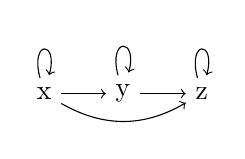
\begin{tikzpicture}[->]
        \node (1) {x};
        \node (2) [right of=1] {y};
        \node (3) [right of=2] {z};
        \path
        (1) edge node {} (2)
        (1) edge [bend right] node {} (3)
        (2) edge node {} (3)
        (1) edge [loop above] node {} (1)
        (2) edge [loop above] node {} (2)
        (3) edge [loop above] node {} (3);
    \end{tikzpicture}
\end{center}
\begin{enumerate}[label=\arabic*)]
    \item $X$ è da considerare come $\Box$ sul frame $(S,R)$
    \item $G$ è da considerare come $\Box$ sul frame $(S,R^*)$
    \item $F$ è da considerare come $\Diamond$ sul frame $(S,R^*)$, quindi $F \varphi = \neg G \neg \varphi$ per ogni formula $\varphi$
    \item U è un connettivo modale 2-ario. è definito da $M \vDash_x U(\varphi, \psi)$ se e solo se
          \begin{enumerate}[label=\alph*)]
              \item $\exists z \in S t.c. (x,z) \in R^*$ e $M \vDash_z \psi$
              \item $M \vDash_y \varphi \forall y \in S t.c. (x,y) \in R^*, (y,z) \in R^*, y \neq z$
          \end{enumerate}
    \item $W(\varphi, \psi)$ se e solo se $U(\varphi, \psi)$ oppure $G \varphi$
    \item $R(\varphi, \psi)$ se e solo se $\neg U(\neg \varphi, \neg \psi)$
\end{enumerate}
Quindi gli unici connettivi modali per definire questa logica solo $X, G$ e $U$.

Gli altri sono esprimibili in termini di questi.
\begin{example}
    Consideriamo la relazione:
    \begin{center}
        $(S,R)$ :
        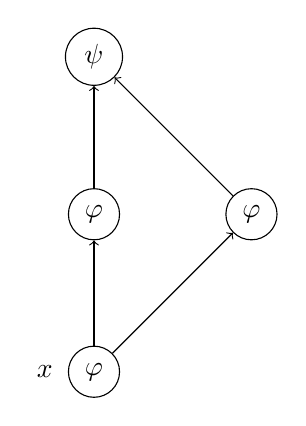
\begin{tikzpicture}[->, baseline=(current bounding box.north), node distance=2cm]
            \node[draw, circle] (1) {$\varphi$};
            \node[left=4mm] at (1) {$x$};
            \node[draw, circle] (2) [above of = 1] {$\varphi$};
            \node[draw, circle] (3) [right of=2] {$\varphi$};
            \node[draw, circle] (4) [above of =2] {$\psi$};
            \path
            (1) edge node {} (2)
            (1) edge node {} (3)
            (2) edge node {} (4)
            (3) edge node {} (4);
        \end{tikzpicture}
        $(S,R^*)$ :
        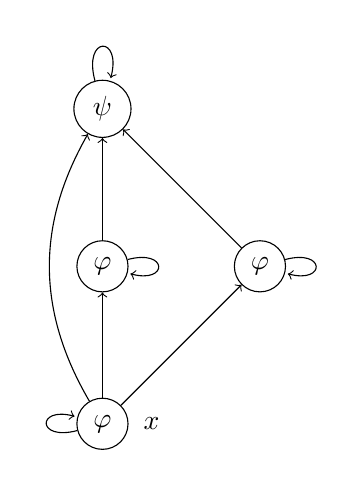
\begin{tikzpicture}[->, baseline=(current bounding box.north), node distance=2cm]
            \node[draw, circle] (1) {$\varphi$};
            \node[right=4mm] at (1) {$x$};
            \node[draw, circle] (2) [above of = 1] {$\varphi$};
            \node[draw, circle] (3) [right of=2] {$\varphi$};
            \node[draw, circle] (4) [above of =2] {$\psi$};
            \path
            (1) edge node {} (2)
            (1) edge [bend left] node {} (4)
            (1) edge node {} (3)
            (2) edge node {} (4)
            (3) edge node {} (4)
            (1) edge [loop left] node {} (1)
            (2) edge [loop right] node {} (2)
            (3) edge [loop right] node {} (3)
            (4) edge [loop above] node {} (4);
        \end{tikzpicture}
        \begin{align*}
             & M \vDash_x X \varphi, \: M \nvDash_x G \varphi              \\
             & M \vDash_x F \varphi, \: M \vDash_x U(\varphi, \psi)        \\
             & M \vDash_x W(\varphi, \psi), \: M \vDash_x R(\varphi, \psi)
        \end{align*}
    \end{center}
\end{example}
\begin{example}
    Consideriamo la relazione:
    \begin{center}
        $(S,R)$ :
        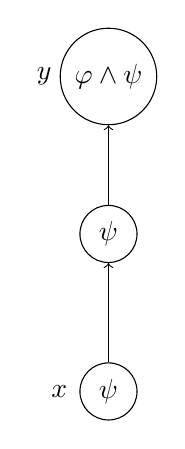
\begin{tikzpicture}[->, baseline=(current bounding box.north), node distance=2cm]
            \node[draw, circle] (1) {$\psi$};
            \node[left=4mm] at (1) {$x$};
            \node[draw, circle] (2) [above of=1] {$\psi$};
            \node[draw, circle] (3) [above of=2] {$\varphi \land \psi$};
            \node[left=6mm] at (3) {$y$};
            \path
            (1) edge node {} (2)
            (2) edge node {} (3);
        \end{tikzpicture}
        $(S,R^*)$:
        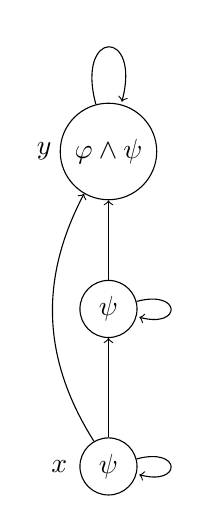
\begin{tikzpicture}[->, baseline=(current bounding box.north), node distance=2cm]
            \node[draw, circle] (1) {$\psi$};
            \node[left=4mm] at (1) {$x$};
            \node[draw, circle] (2) [above of=1] {$\psi$};
            \node[draw, circle] (3) [above of=2] {$\varphi \land \psi$};
            \node[left=6mm] at (3) {$y$};
            \path
            (1) edge node {} (2)
            (1) edge [bend left] node {} (3)
            (2) edge node {} (3)
            (1) edge [loop right] node {} (1)
            (2) edge [loop right] node {} (2)
            (3) edge [loop above] node {} (3);
        \end{tikzpicture}
        \begin{align*}
             & M \vDash_x X \psi, \: M \vDash_x G \psi, \: M \vDash_y G \psi            \\
             & M \nvDash_x X \varphi, \: M \nvDash_x G \varphi, \: M \vDash_y G \varphi \\
             & M \vDash_x F \varphi, \: M \vDash_x U(\psi, \varphi)                     \\
             & M \vDash_x W(\psi, \varphi), \: M \vDash_x R(\varphi, \psi)
        \end{align*}
    \end{center}
    $\varphi R \psi : \neg U(\neg \varphi, \neg \psi)$.

    $M \vDash_x \neg U(\neg \varphi, \neg \psi) \iff M \nvDash_x U(\neg \varphi, \neg \psi) \iff $

    o $\forall z \in S$ t.c $(x,z) \in R^*, M \vDash_z \psi$

    o $\forall z \in S$ t.c $(x,z) \in R^*. M \vDash_z \neg \psi, \exists y \in S$ t.c $(x,y) \in R^*, (y,z) \in R^*, y \neq z, M \vDash_y \varphi$

    $\psi$ deve essere vere fino al punto in cui inizia ad essere vera $\varphi$ ($\varphi$ rilascia $\psi$)
\end{example}

\newpage

\subsection{Logiche Temporali CTL (Computation Tree Logic)}
In queste logiche modali, quantifichiamo sui cammini del grafo diretto che rappresenta il frame $(S,R)$.

I connettivi modali sono:
\begin{gather*}
    AX, EX, AF, EF, AG, EG \qquad \text{(1-ari)}\\
    AU, EU \qquad \text{(2-ari)}
\end{gather*}
$A$ sta per "Along all paths", $E$ sta per "along at least one path (there Exists)"
\subsubsection{Semantica}
\begin{enumerate}[label=\arabic*)]
    \item $M \vDash_w AX \psi $ se e solo se $\forall v \in S$ t.c $(w,s) \in R \text{(c'è un arco)} , M \vDash_s \psi$, ossia si comporta come $\Box$ su $(S,R)$
    \item $M \vDash_w EX \psi $ se e solo se $\exists s \in S$ t.c $(w,s) \in R \text{(c'è un arco)} , M \vDash_s \psi$, ossia si comporta come $\Diamond$ su $(S,R)$
    \item $AG$ si comporta come $\Box$ su $(S,R^*)$
    \item $M \vDash_w EG \varphi$ se e solo se esiste un cammino $s_0 := w \to s_1 \to s_2 \to \ldots $ in $(S,R)$ tale che $M \vDash_{s_i} \varphi$ (lungo il cammino)
    \item $M \vDash_w EU (\varphi, \psi)$ se e solo se esiste un cammino in $(S,R)$ tale che $M \vDash_{s_i} U(\varphi, \psi)$ (lungo il cammino, possiamo intenderlo come sotto-frame)
\end{enumerate}
Analogamente si definiscono gli altri connettivi modali.
\begin{example}
    Nei grafi:
    \begin{center}
        \begin{tikzpicture}[->]
            \node (1) {$(S_0)\circ$};
            \node (2) [below of=1] {$\circ$};
            \node (3) [right of =2] {$\circ$};
            \node (4) [below of=2] {$\circ$};
            \node (5) [right of = 4] {$\varphi$};
            \node (6) [right of = 5] {$\varphi$};
            \node (7) [right of = 6] {$\varphi$};
            \node (8) [below of=4]{$\varphi$};
            \node (9) [right of = 8] {$\circ$};
            \node (10) [right of = 9] {$\circ$};
            \node (11) [right of = 10] {$\circ$};
            \node (12) [right of = 11] {$\circ$};
            \node (13) [below of=8] {$\circ$};
            \node (14) [below of=9] {$\varphi$};
            \node (15) [below of=14] {$\circ$};

            \path
            (1) edge node {} (2)
            (1) edge node {} (3)
            (2) edge node {} (4)
            (3) edge node {} (5)
            (3) edge node {} (6)
            (3) edge node {} (7)
            (4) edge node {} (8)
            (4) edge node {} (9)
            (5) edge node {} (10)
            (6) edge node {} (11)
            (7) edge node {} (12)
            (8) edge node {} (13)
            (9) edge node {} (14)
            (14) edge node {} (15);

        \end{tikzpicture}
        $M \vDash_{S_0} AF \varphi$
        \begin{tikzpicture}[->]
            \node (1) {$(S_0)\circ$};
            \node (2) [below of=1] {$\circ$};
            \node (3) [right of =2] {$\circ$};
            \node (4) [below of=2] {$\circ$};
            \node (5) [right of = 4] {$\circ$};
            \node (6) [right of = 5] {$\circ$};
            \node (7) [right of = 6] {$\circ$};
            \node (8) [below of=4]{$\circ$};
            \node (9) [right of = 8] {$\varphi$};
            \node (10) [right of = 9] {$\circ$};
            \node (11) [right of = 10] {$\circ$};
            \node (12) [right of = 11] {$\circ$};
            \node (13) [below of=8] {$\circ$};
            \node (14) [below of=9] {$\circ$};
            \node (15) [below of=14] {$\circ$};

            \path
            (1) edge node {} (2)
            (1) edge node {} (3)
            (2) edge node {} (4)
            (3) edge node {} (5)
            (3) edge node {} (6)
            (3) edge node {} (7)
            (4) edge node {} (8)
            (4) edge node {} (9)
            (5) edge node {} (10)
            (6) edge node {} (11)
            (7) edge node {} (12)
            (8) edge node {} (13)
            (9) edge node {} (14)
            (14) edge node {} (15);

        \end{tikzpicture}
        $M \vDash_{S_0} EF \varphi$\\
        \begin{tikzpicture}[->]
            \node (1) {$(S_0)\varphi$};
            \node (2) [below of=1] {$\varphi$};
            \node (3) [right of =2] {$\varphi$};
            \node (4) [below of=2] {$\varphi$};
            \node (5) [right of = 4] {$\varphi$};
            \node (6) [right of = 5] {$\varphi$};
            \node (7) [right of = 6] {$\varphi$};
            \node (8) [below of=4]{$\varphi$};
            \node (9) [right of = 8] {$\varphi$};
            \node (10) [right of = 9] {$\varphi$};
            \node (11) [right of = 10] {$\varphi$};
            \node (12) [right of = 11] {$\varphi$};
            \node (13) [below of=8] {$\varphi$};
            \node (14) [below of=9] {$\varphi$};
            \node (15) [below of=14] {$\varphi$};

            \path
            (1) edge node {} (2)
            (1) edge node {} (3)
            (2) edge node {} (4)
            (3) edge node {} (5)
            (3) edge node {} (6)
            (3) edge node {} (7)
            (4) edge node {} (8)
            (4) edge node {} (9)
            (5) edge node {} (10)
            (6) edge node {} (11)
            (7) edge node {} (12)
            (8) edge node {} (13)
            (9) edge node {} (14)
            (14) edge node {} (15);

        \end{tikzpicture}
        $M \vDash_{S_0} AG \varphi$
    \end{center}
\end{example}
\newpage
\subsection{Logiche CTL*}
Le logiche CTL* hanno la stessa semantica delle LTL, a cui aggiungiamo i quantificatori $A$ "Along all paths" ed $E$ "Along at least one path".

Quindi CTL* contiene LTL e CTL.

In LTL possiamo esprimere l'affermazione "su tutti i cammini in cui appare $\psi$ appare anche $\varphi$":
\begin{equation*}
    F\varphi \implies F \psi
\end{equation*}
in CTL non possiamo esprimerla, ma in CTL* si, dato che contiene LTL.
\begin{equation*}
    E(GF\varphi)
\end{equation*}
ovviamente tale affermazione non è esprimibile in LTL a meno che il frame $(S,R)$ non abbia un solo cammino.

Non è esprimibile neanche in CTL; infatti ha un altro significato:
\begin{example} in CTL:
    \begin{center}
        \begin{tikzpicture}[->]
            \node (1) {$(S_0)\varphi$};
            \node (2) [below of=1] {$\circ$};
            \node (3) [right of =2] {$\circ$};
            \node (4) [below of=2] {$\circ$};
            \node (5) [right of = 4] {$\varphi$};
            \node (6) [right of = 5] {$\varphi$};
            \node (7) [right of = 6] {$\varphi$};
            \node (8) [below of=4]{$\varphi$};
            \node (9) [right of = 8] {$\circ$};
            \node (10) [right of = 9] {$\circ$};
            \node (11) [right of = 10] {$\circ$};
            \node (12) [right of = 11] {$\circ$};
            \node (13) [below of=8] {$\circ$};
            \node (14) [below of=9] {$\varphi$};
            \node (15) [below of=14] {$\circ$};

            \path
            (1) edge node {} (2)
            (1) edge node {} (3)
            (2) edge node {} (4)
            (3) edge node {} (5)
            (3) edge node {} (6)
            (3) edge node {} (7)
            (4) edge node {} (8)
            (4) edge node {} (9)
            (5) edge node {} (10)
            (6) edge node {} (11)
            (7) edge node {} (12)
            (8) edge node {} (13)
            (9) edge node {} (14)
            (14) edge node {} (15);

        \end{tikzpicture}\\
        $M \vDash_{S_0} EG(EF \varphi)$ in CTL
    \end{center}
\end{example}
\newpage
\subsection{Model Checking}
\begin{example}
    Quando più processi eseguono in contemporanea, se condividono una risorsa potrebbe essere necessario assicurare che non vi accedano nello stesso momento.

    Ad esempio non vorremmo che più di un processo modifichi un file nello stesso momento.

    Definiamo delle "sezioni critiche" per ogni codice del processo e le disponiamo in modo che due processi non si trovino nella stessa sezione critica nello stesso momento.

    Vogliamo che valga la seguente proprietà:

    \textbf{Sicurezza}: "Un processo alla volta può stare nella sezione critica"

    per due processi $P1$ e $P2$, consideriamo le variabili:
    \begin{itemize}
        \item $n_1 := $ "processo 1 non sta in stato critico"
        \item $n_2 := $ "processo 2 non sta in stato critico"
        \item $c_1 := $ "processo 1 sta in stato critico"
        \item $c_2 := $ "processo 2 sta in stato critico"
        \item $t_1 := $ "processo 1 prova a entrare in stato critico"
        \item $t_2 := $ "processo 2 prova a entrare in stato critico"
    \end{itemize}

    Sicurezza è esprimibile in LTL come: $\varphi_1 = G\neg (c_1 \land c_2)$ ossia $M \vDash_{S_0} G\neg (c_1 \land c_2)$.

    Un'altra condizione che vogliamo sia verificata è:

    \textbf{Vitalità}: "Ogni volta che un processo chiede di entrare nella sua sezione critica, gli sarà permesso in un altro momento"

    Questa condizione è esprimibile in CTL come:
    \begin{equation*}
        M \vDash_{S_0} (AGt_1 \implies EF c_1) \land (AGt_2 \implies EF c_2) \equiv \varphi_2
    \end{equation*}
    considerando il seguente frame:
    \begin{center}
        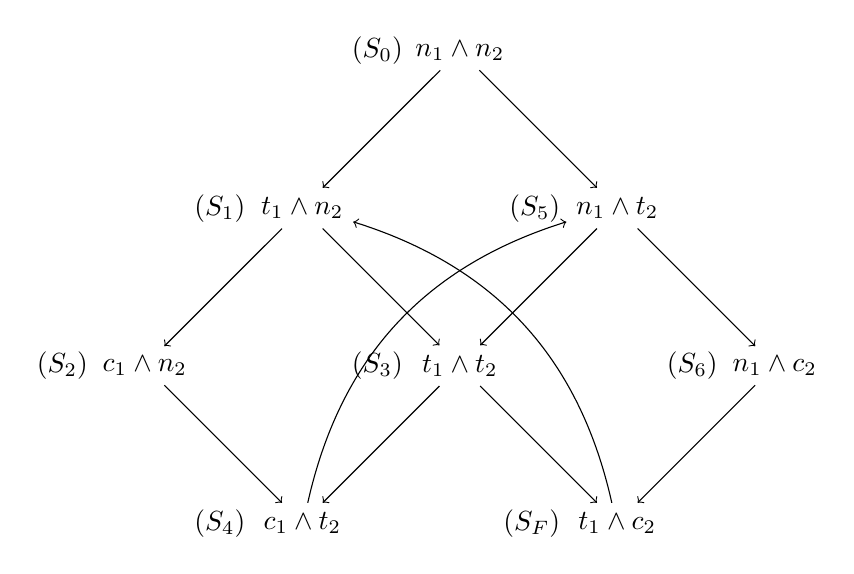
\begin{tikzpicture}[->, node distance=2cm]
            \node (1) {$n_1 \land n_2$};
            \node[left=6mm] at (1) {$(S_0)$};
            \node (2) [below of=1, left of=1] {$t_1 \land n_2$};
            \node[left=6mm] at (2) {$(S_1)$};
            \node (3) [below of = 1, right of =1] {$n_1 \land t_2$};
            \node[left=6mm] at (3) {$(S_5)$};
            \node (4) [below of=2, left of =2] {$c_1 \land n_2$};
            \node[left=6mm] at (4) {$(S_2)$};
            \node (5) [below of =2, right of = 2] {$t_1 \land t_2$};
            \node[left=6mm] at (5) {$(S_3)$};
            \node (6) [below of=3, right of = 3] {$n_1 \land c_2$};
            \node[left=6mm] at (6) {$(S_6)$};
            \node (7) [below of =4, right of = 4] {$c_1 \land t_2$};
            \node[left=6mm] at (7) {$(S_4)$};
            \node (8) [below of=5, right of=5]{$t_1 \land c_2$};
            \node[left=6mm] at (8) {$(S_F)$};

            \path
            (1) edge node {} (2)
            (1) edge node {} (3)
            (2) edge node {} (4)
            (2) edge node {} (5)
            (3) edge node {} (5)
            (3) edge node {} (6)
            (4) edge node {} (7)
            (5) edge node {} (7)
            (5) edge node {} (8)
            (6) edge node {} (8)
            (7) edge[bend left] node {} (3)
            (8) edge [bend right] node {} (2);
        \end{tikzpicture}\\
        abbiamo che vale $M \vDash_{S_0} \varphi_1 \land \varphi_2$
    \end{center}
\end{example}
\end{document}